\chapter[Sequential models: RNN, LSTM, GRU, Transformers]{Sequential and Attention models: RNN, LSTM, GRU, Transformers}
%--------------------------------------------------------

%-----------------------Sequence models (I gruppo di slides)------------
\begin{quotation}
    \noindent
    \textsf{In this chapter we will discuss about some tasks that according to their features requires special neural network architectures that are something different with respect to the model we have already seen talking about MLP and ConvNet for computer vision activities. We are talking about \textit{Recurrent Neural Network (RNN)}, such models are used in order to perform computation on  \textit{time series data}. \textbf{Time} is the new component to handle. The related tasks include: speech recognition, music generation, DNA sequence analysis and so on. After some prerequisites, we are introducing RNN and more robust architectures (\textit{LSTM, GRU}). Finally the state-of-art architecture for NLP is analyzed (\textit{Transformer}).  
    }
\end{quotation}

\begin{figure}[h]
    \centering
    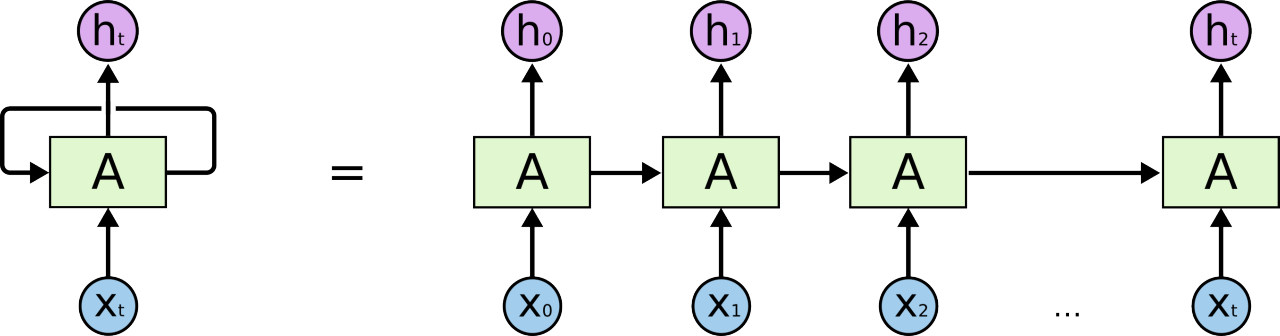
\includegraphics[scale=0.3]{img/rnn_1.png}
\end{figure}

\section{Notation}
In order to introduce some \textbf{notation}, we use a practical example. In the field of information extraction in the context of \textit{Natural Language processing (NLP)}, there is a sub-task which is called \textbf{Named entity recognition}, this deals with the classification of the name appearing in a sentence according to predetermined categories.
Suppose you want to recognize the person name in the sentence:
\begin{center}
    \textit{Harry Potter and Hermione Granger invented a new spell}
\end{center}
This is a sequence of words constituting a phrase. We need a notation in order to handle the concept of \textit{sequentiality}. One possibility is to use for the words, which will be the input of our models (anyhow they are made), the notation
\begin{equation*}
    x=\{x_{(1)}\quad x_{(2)} \quad ... \quad x_{(T_x)}\}
\end{equation*}  
Indicating with an index the \textit{time at which the word appear in the sentence}. The size of the input sample $x$ is $T_x$. The same reasoning holds for the output $y$, which is suggesting us, the words related to name of person. In the specific case we will have
\begin{equation*}
    y=\{y_{(1)}, y_{(2)}, \dots, y_{(T_y)}\} = \{1,1,0,1,1,0,0,0,0\}
\end{equation*}
Since \textit{Harry Potter} and \textit{Hermion Granger} are the names in the given sequence. It is not said that $T_x$ and $T_y$ are of the same length. The concept of \textbf{time} is a novelty with respect to the other tasks we have seen. Sequentiality makes necessary the introduction of new aspects we have not considered till now. Let us start!

\section{Representing words}
It is not a novelty if we say that Neural networks manage effectively numbers by doing several forms of computation in order to perform their task. Well, even in the presence of sequential data, we have to map them in some "numeric space", first of all the \textbf{words}. \\

When we are dealing with NLP, mostly, there is a \textbf{dictionary} with a great number of words which can be used in the analysis. Then, if we have examples made up of phrases, each word is mapped into a \textit{sparse vector} in which \textbf{only the number at the position where the word itself is located in the vocabulary is one}, all the other numbers are 0. For this reason such an encoding is called \textbf{one-hot encoding}. 
Such a work is carried out after that the sentences have been \textbf{tokenized}\footnote{
    Sometimes, for certain types of computation, the \textbf{stemming} is preferred; this is the process by which each word is recasted to its \textit{root form}.
}. \\
To tell the truth the architectures we are going to see, do not take into account this sparse representation, at least directly. Differently, often the words during the training of \textit{language models} are mapped into an \textit{hyperdimensional dense space} in the so-called \textbf{word embeddings} which are succint synthesis of the general meaning for a certain word. Such encoding can be pretrained or fine tuned or made by scratch in some cases, being included into the \textit{trainable parameters}. Anyway, \textit{one-hot encodings} are important since they are fed into an \textit{embedding lookup module} which will provide the inputs $x$ to the NN. To conclude this part, let us provide an example. We want the one-hot encodings for the word \textit{cat}, while the voabulary is: 
\begin{align*}
    \text{Vocabulary} =\{ a,\ aaron, \ ..., \  aerospace, \ cat, \ ..., \  zulu\}
\end{align*}
The one-hot encoding is:
\begin{equation*}
    [0, \ 0, \ ... \ 0, \ 1, \ ..., 0]
\end{equation*}

\section{Recurrent Neural Networks (RNN)}
\subsection{Motivations for introducing a novel architecture}
Everytime we have to introduce a new architecture, it is quite natural asking ourself: \textit{Can we use, instead, the architectures we already have?} There are several reasons for which the answer is NO.
\begin{enumerate}
    \itemsep-0.2em
    \item In models dealing with sequential data, the \textbf{size} of input/output \textbf{can be different} in different samples.
    \item Standard NNs do not share the features learned across the different position of the sequence; 
    \item Standard NNs, first of all, do not include \textit{ memory mechanisms} which are fundamental here, due to the presence of \textit{sequentiality}
\end{enumerate}

\subsection{Recurrent neurons and layers}
Up to now we have seen models where the outputs flowed only in one direction: forward. A \textbf{recurrent neural network} has more or less the same structure of a Feed-forward Neural Network, except the fact it have \textbf{backward connections}. \\
The simplest possible RNN is the one made up of \textit{one neuron} that receive the input, produce the output and send its output, or in more complex situations, its \textbf{hidden state}, back to itself. When the first input is received this output/hidden state is usually initialized to 0 since the network has not already produced any output. As showed in \Cref{fig:r_neuron} the recurrent neuron can be represented \textit{against the time axis} in the so-called \textbf{unrolled representation} (it's the same recurrent neuron once per time step).

\begin{figure}[h]
    \centering
    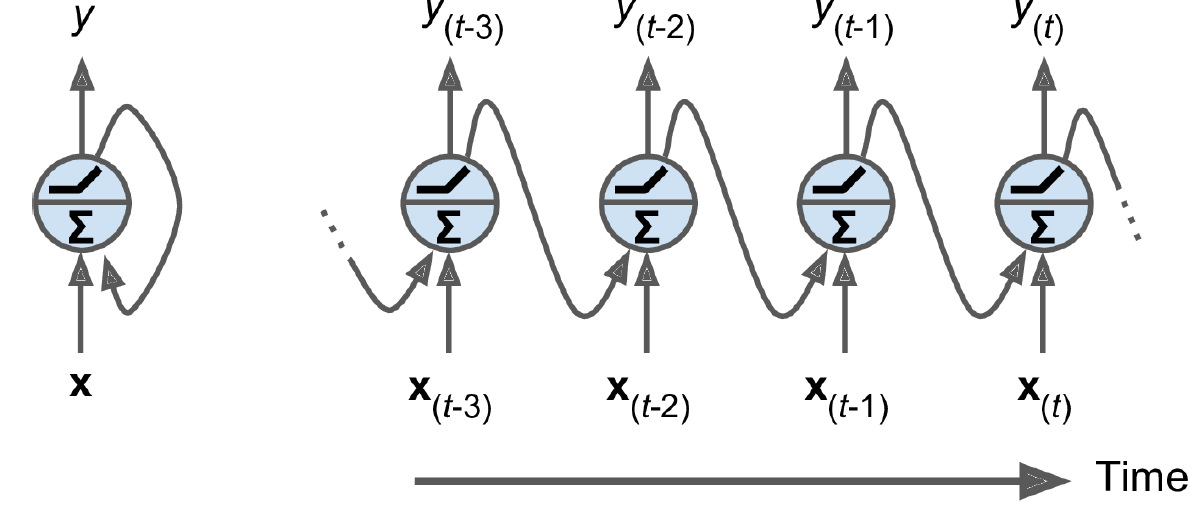
\includegraphics[scale=0.5]{img/rnn.png}
    \caption{Recurrent neuron}
    \label{fig:r_neuron}
\end{figure}
\noindent
Here, it is even more clear that for each time instant the neuron, receives not only the input $x$ but also another information coming from past computations. The output of such a \textit{tiny network} is simply a scalar.\\
It is quite simple to extend the reasoning we have done for a \textbf{layer recurrent neurons} where each neuron receives the input and the \textbf{backward information}. Here the output is a vector, since there many neurons. A \textit{recurrent layer} together with its unrolled representation is showed in the \Cref{fig:r_layer}.

\begin{figure}
    \centering
    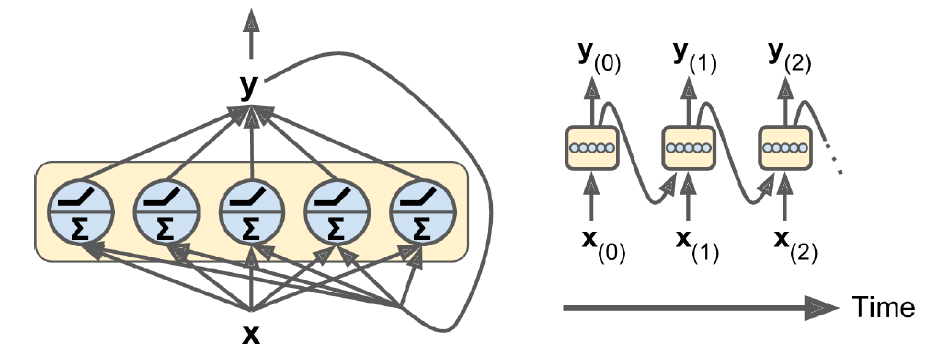
\includegraphics[scale=0.7]{img/rnn_layer.png}
    \caption{Recurrent layer}
    \label{fig:r_layer}
\end{figure}

Since the output of a recurrent neuron at time step $t$ is a function of all the inputs from previous time steps, this is the reason why we refer to recurrent architecture by using the term \textbf{memory cell}. In the examples we have analyzed of recurrent neuron and layer, we have assumed that the backward information was the output, in more complex architectures this is not the case, but we call it \textbf{hidden state} (see \cref{fig:rnn_hidden}), we are indicating it with the notation $h^{<t>}$.\\
Each neuron has \textbf{three sets of weights}: 
\begin{enumerate}
    \itemsep-0.2em
    \item $\mathbf{w}_{hx}$ from the input to the hidden state; 
    \item $\mathbf{w}_{hh}$ from one hidden state and the following; 
    \item $\mathbf{w}_{yh}$ from the hidden state to the output
\end{enumerate} 
Since we have multiple neurons we can group such weights in matrices, like we did for feedforward architectures. Then, we have $\mathbf{W}_{hx}$, $\mathbf{W}_{hh}$ and $\mathbf{W}_{ya}$. \\

\hrule
\vspace{0.2cm}
\noindent
\textsc{\large What about the training of an RNN?}\\
 We have to use a trick which we have already  seen in some sense, that is, we have to unroll the network through the time and then apply, after the forward pass, the backward propagation. Let us clarify in details these aspects.

\subsubsection{Forward propagation}
The following are the steps to perform in order to carry out the \textbf{forward propagation}, the most general case is considered when the hidden state $h$ is different with respect to the output $y$. The equations for the hidden state and for the output are respectively:
\vspace{-0.2cm}
\begin{align}
    \large
    &\mathbf{h}_{(t)}=g_h(\mathbf{W}_{hh} \mathbf{h}_{(t-1)}+\mathbf{W}_{hx}\mathbf{x}_{(t)}+\mathbf{b}_h) \label{eq:hidden_eq}\\
    &\hat{\mathbf{y}}_{(t)}=g_o(\mathbf{W}_{yh}\mathbf{h}_{(t)}+\mathbf{b}_y)\label{eq:output_eq}
\end{align}
where $g_h$, $g_o$ are the activation functions related to, respectively, the hidden state and the output, while $\mathbf{b}_h$, $\mathbf{b}_o$ are the bias vectors. A simplified notation can be used if the two matrices of the hidden state are collapsed into 
\begin{equation*}
    \mathbf{W} = [\mathbf{W}_{hh} \quad \mathbf{W}_{hx}]
\end{equation*} 
so that the \Cref{eq:hidden_eq} becomes: 
\begin{equation*}
    h_{(t)}=g_h(\mathbf{W}\cdot[\mathbf{h}_{(t-1)} \quad \mathbf{x}_{(t)}]^T+\mathbf{b}_h)
\end{equation*}
If we had considered all of the examples of the mini-batch on which we compute the forward pass the all of the involved quantities would have been matrices, in particular $\mathbf{H}_{(t)}$, $\mathbf{X}_{(t)}$ and $\mathbf{Y}_{(t)}$.


\subsubsection{Backward propagation}
The strategy according to we can update the weights in an RNN, is called \textbf{Backpropagation through time (BPTT)}. Like in a regular BP, there is first a forward step through the unrolled network, then a loss function is computed according to the outputs. In particular we have that the loss $\text{J}(\hat{y},y)$ will be: 
\begin{equation}
    \text{J}(\hat{y},y)=\sum_{t=1}^{T_y} {\text{Loss}_{(t)}(\hat{y}_{(t)}, y_{(t)})}
\end{equation}
The derivatives (gradients) of such a cost function are computed and backpropagated through the unrolled network. In some cases, the cost function could depend only on a subset of outputs. It should be clear that, since the unrolled network is nothing but the same architecture repeated over time, the weights are the same for each \textit{time step} or \textit{frame}. The \Cref{fig:BPTT} shows the BPTT process, the dashed arrows represent the forward pass, the solid ones the backward pass. Note that here is considered the case where the cost function accounts only for three out of five of the outputs, moreover the cost function is indicated with C while considering together the whole mini-batch.

\begin{multicols}{2}
    \begin{figure}[H]
        \centering
        \label{fig:BPTT}
        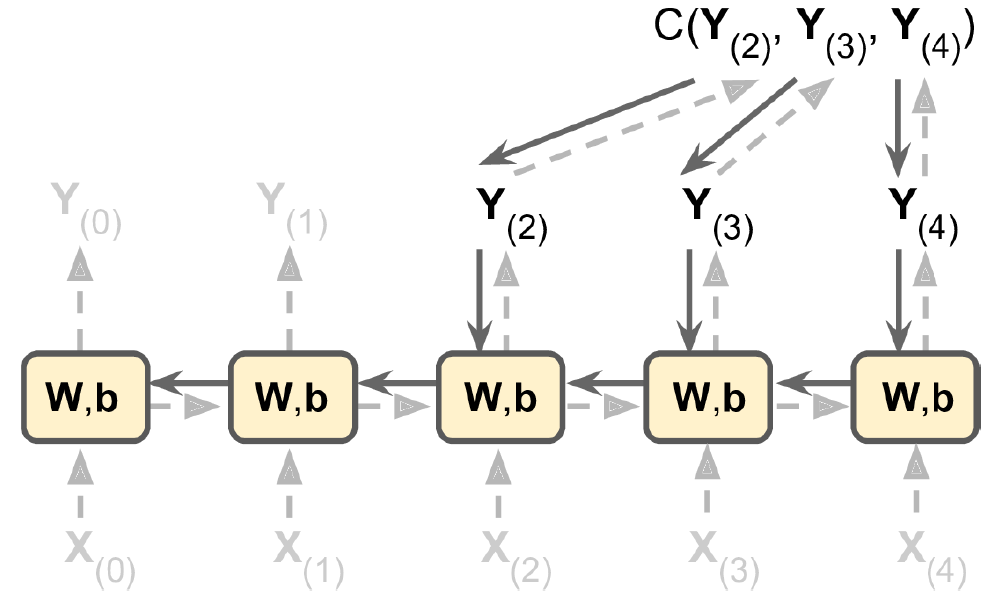
\includegraphics[scale=0.35]{img/BPTT.png}
        \caption{\textit{Backpropagation through time}}
    \end{figure}
    \newcolumn
    \begin{figure}[H]
        \centering
        \label{fig:rnn_hidden}
        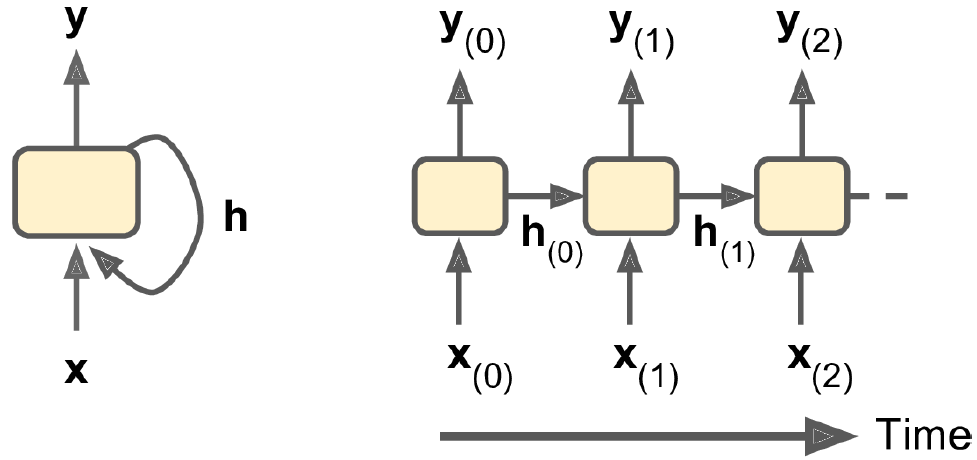
\includegraphics[scale=0.4]{img/rnn_hidden.png}
        \caption{\textit{Hidden state $\ne$ Output}}
    \end{figure}
\end{multicols}

\subsection{RNN architectures}
In the introduction we have mentioned the fact that $T_x$ could be different than $T_y$, in the great majority this is the case. Several combinations are possible. The \Cref{fig:RNN_archs} shows the different cases, including the encoder-decoder architecture.
\vspace{-0.2cm}
\subsubsection{Sequence-to-sequence}\vspace{-0.2cm}
In this case there is a sequence as input and a sequence for output. Such a network is useful for example for \textit{predicting time series} such as stock prices.
\vspace{-0.2cm}
\subsubsection{Sequence-to-vector}\vspace{-0.2cm}

In this case a sequence of data is fed into the network, but the output are all ignored except the last one. This is common when an RNN is used for \textit{sentiment analysis}. For example the output is a sequence of words constituting a film review the output is a score between -1 [hate] and 1[love].
\vspace{-0.2cm}
\subsubsection{Vector-to-sequence}\vspace{-0.2cm}

When you feed the network with the \textit{same vector} over and over and the output is a sequence, you build a \textit{vector-to-sequence} RNN. An example is the \textbf{image captioning} (on which we dedicate a section) where the input is, for example, the feature vector coming from a ConvNet, the output is a sentence (sequence of words) containing a description for that image.

\subsubsection{Encoder-Decoder}
An \textbf{Encoder-Decoder RNN} is a quite particular architecture made up of: (i) a sequence-to-vector structure followed by a (ii) vector-to-sequence structure. This is one of the first architectures used in the field of \textit{Neural Machine Translation (NMT)}. Here, the encoder (sequence2vector) is converting the input sequence into a \textbf{single vector representation}, this is the input of the decoder (vector-to-sequence) part which is decoding  into a sentence in another language. This works much better than translating a sentence on fly by using a single sequence-to-sequence architectures, since the meaning of the first word could depend from the following. Usually the architecture is a little bit more complex with respect to the one showed in \Cref{fig:RNN_archs} how we will see.

\begin{figure}[h] 
    \centering
    \label{fig:RNN_archs}   
    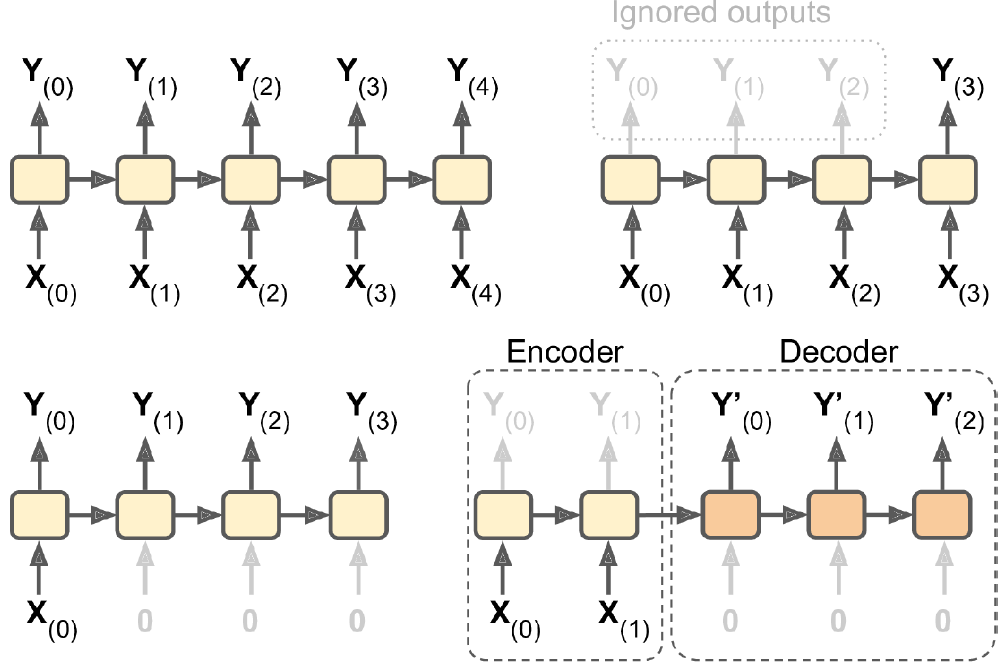
\includegraphics[scale=0.5]{img/rnn_archs.png}
    \caption{RNN architectures}
\end{figure}

\vspace{-1cm}
\subsection{Bidirectional RNN}
At each time step a usual recurrent layer only looks at past and present inputs before generating its outputs. In some applications it is preferable that to look ahead the next words before giving the output. For example in order to well encode the word "queen" in the sentences "The Queen of the United Kingdom" and "The queen of the hearts", we have to look ahead the other words since the meaning of the word is completely different in the two situations. In order to solve this problem we have to run in parallel \textbf{two recurrent layers} fed with the same input sequence, the difference is that one is reading from the beginning to the end, the other from the end to the beginning. Then, "simply" the output is \textit{combined} at each time step. The resulting architecture is the so-called \textbf{bidirectional RNN}.

\begin{figure}[h]
    \centering
    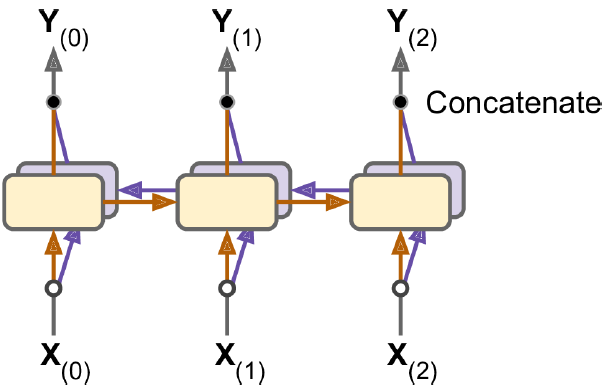
\includegraphics[scale=0.5]{img/rnn_bidir.png}
    \caption{Bidirectional recurrent layer}
\end{figure}

\subsection{Deep RNN}
It is a common pratctice to stack several RNN cells, what you obtain is a \textit{Deep RNN} architecture. The figure shows a deep recurrent network together with its unrolled version.

\begin{figure}[h]
    \centering
    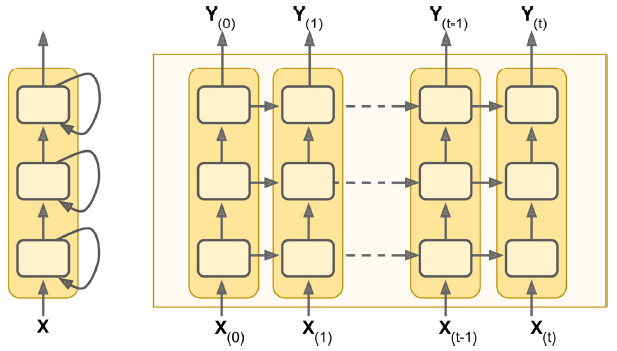
\includegraphics[scale=0.7]{img/rnn_deep.png}
    \caption{A \textit{Deep RNN}}
\end{figure}
\noindent
What changes in the notation is that all the showed equations for feedforward and backward propagation have another index indicating the layer. Clearly the matrices \textbf{W} are different according to the layer of the deep RNN.

\section{Language Modeling with RNN}
Before entering in the discussion on \textit{"How RNN can be used for NLP\footnote{
    Natural Language Processing (NLP tasks)
}"}. It is important to understand, in general what is the idea behind having a \textbf{model for the language}. The \textbf{language modeling} can be seen in a general framework where it is required to \textit{predict the probability of a certain sequence of words}. For example, between these two sentences:
\begin{center}
    The apple and pair salad\\
    \underline{The apple and pear salad}
\end{center} 
what is the \textbf{most probable}? Clearly the second! The task is formulated in general as \textbf{predicting the next word given a set of previous words}. In formula:
\begin{equation}
    P(w_1, w_2,...,w_T)=P(w_1) \cdot P(w_2|w_1)\cdot \dots \cdot P(w_T|w_1,...,w_{T-1})
\end{equation}
So the probability of a certain sequence is given by the \textbf{conditional probabilities} of its own words. For such models the \textbf{training set} are \textit{large corpora}, entire repository with books, paper and so on. While the \textbf{objective of the training} is \textit{minimizing the prediction error on the next word}. \\
This is the right place to highlight that for each sequence a special token of <EOS> (End of sequence is used), in order to split a sequence from another.\\
In this context the \textbf{role of an RNN architecture} is to predict, step-by-step, the probability for the vocabulary words to be the next word, given a sequence of previous words. Now, there are two common situations:
\begin{enumerate}
    \item The \textbf{Word Embeddings} are pretrained, and eventually only fine-tuned, on the current sequences; embedding like \textsc{Word2Vec} can be used in this case; 
    \item The \textbf{Word Embeddings} are part of the trainable parameters.
\end{enumerate}
\noindent
In the former case only the weights and biases are update by backward propagation, in the latter case, also the vocabulary embeddings are updated in order to obtain a general representation for the meaning of a certain word.

\subsection{Training an RNN language model}
The sentences of the training set are passed through the network, at each step an output probability is computed, using a softmax on the output vector $\mathbf{\hat{y}}_{(t)}$. The process is going on until the token <EOS> is reached. Such a situation is showed in the figure below: 

\begin{multicols}{2}
    \begin{figure}[H]
        \centering
        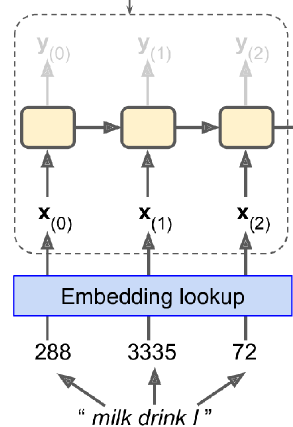
\includegraphics[scale=0.8]{img/rnn_language.png}
    \end{figure}
    Note that the hidden state are updated using the word embeddings obtained by passing the words one-hot encodings through a lookup module.  After this forward propagation step a \textit{cross-entropy loss} is computed comparing the generated and real next word of the sentences, then weights are updated. More specifically the required steps are:
    \begin{enumerate}
        \itemsep-0.2em
        \item[\ding{202}] Update the hidden state $\mathbf{h}_{(t)}$ using $\mathbf{h}_{(t-1)}$ and $\mathbf{e}_{(t)}$ (embedding); 
        \item[\ding{203}] An output $\mathbf{\hat{y}}_{(t)}$ is computed using the hidden state at time $t$ linearly combined and passed through an activation function, this is mapped into a probability vector $\mathbf{p}_{(t+1)}$ using the softmax; 
        \item[\ding{204}] The loss is computed for each time step using the real word $w_{(t+1)}$ and the computed probability distribution using the cross-entropy\footnote{
            What is the sense behind the notation $\mathbf{p}_{t+1}\mathbf[w_{t+1}]$? $\mathbf{p}_{t+1}$ is the probability distribution for the next word, while $w_{t+1}$ is the true next word. If such an index is very low, this result in a bad prediction for the network, taking $-log(\mathbf{p}_{t+1}\mathbf[w_{t+1}])$ increase the loss contribution of a number which is bigger when the probability is low.
        }:
        \begin{equation}
            \text{Loss}_t = -\log(\mathbf{p}_{t+1}\mathbf[w_{t+1}])            
        \end{equation}
        the final loss is obtained summing up these contributions for all time steps.
        \item[\ding{204}] BPTT is performed in order to update the weight matrices $\mathbf{W}_h$ and $\mathbf{W}_y$ and biases vector $\mathbf{b}_h$ and $\mathbf{b}_y$. 
    \end{enumerate}
\end{multicols}

\subsection{Use case: Sentence generation}
After the training of such a model, how can we use it? \textbf{Sentence generation} is one of the tasks for which such a model can be used. The detailed procedure is: 
\begin{enumerate}
    \itemsep-0.2em
    \item We \textbf{initialize the state $\mathbf{h}_0$} which may be zero or a learned value, while as first input of the sentence we pass the embedding of a <SOS>\footnote{
        \textit{Start of Sequence} or \textit{Start of Sentence}
    } token; 
    \item In order to \textbf{obtain the first word}, the hidden state corresponding to $\mathbf{h}_0$ is computed, and then the softmax-probability on the logit outputs.
    \item Now, we have  to \textbf{select a word}, this can be done using several strategies: (i) We take the argmax, (ii) we sample the probability distribution. (There is another more complicated approach (\textit{Beam Search}) which is not treated here).
    \item The selected $w_1$ is used as an input (we mean $\mathbf{E}[w_1]$ where $E$ is the \textbf{embedding matrix}) for the next step.
    \item Such steps are repeated till the token <EOS> is not predicted, this token (the same holds for <SOS> (or <BOS>)) in included in the embedding matrix.
\end{enumerate}
The following figure depicts effectively the process we have just explained: 

\begin{figure}[h]
    \centering
    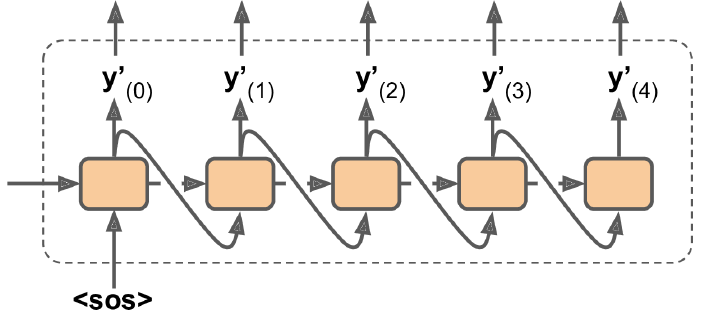
\includegraphics[scale=0.6]{img/sentence_genesis.png}
\end{figure}

\section{Issues with RNN training}

\begin{multicols}{2}
    \noindent
    The main problem in the training of basic RNN architectures is the  \textbf{short-term memory}: due to the way the information are passing through the network, \textit{some information is lost at each time step}, after a while the RNN hidden state has actually no trace of the first input. Image you are reading a sentence, and at the end you have not understood due to the fact you forgot the first part. In order to tackle this problem different types of \textbf{cells} have been introduced. Such cells have some \textbf{long-term memory} that over the time have made unused the basic cell. 

    In the figure a basic cell is showed. This is nothing but the graphical representation of the formulas (\ref{eq:hidden_eq})-(\ref{eq:output_eq}).\\

    In the article \citeauthor{pascanu2013difficulty}, \textit{\citetitle{pascanu2013difficulty}}, \citedate{pascanu2013difficulty}, \cite{pascanu2013difficulty} such issues are better explained.

    \begin{figure}[H]
        \centering
        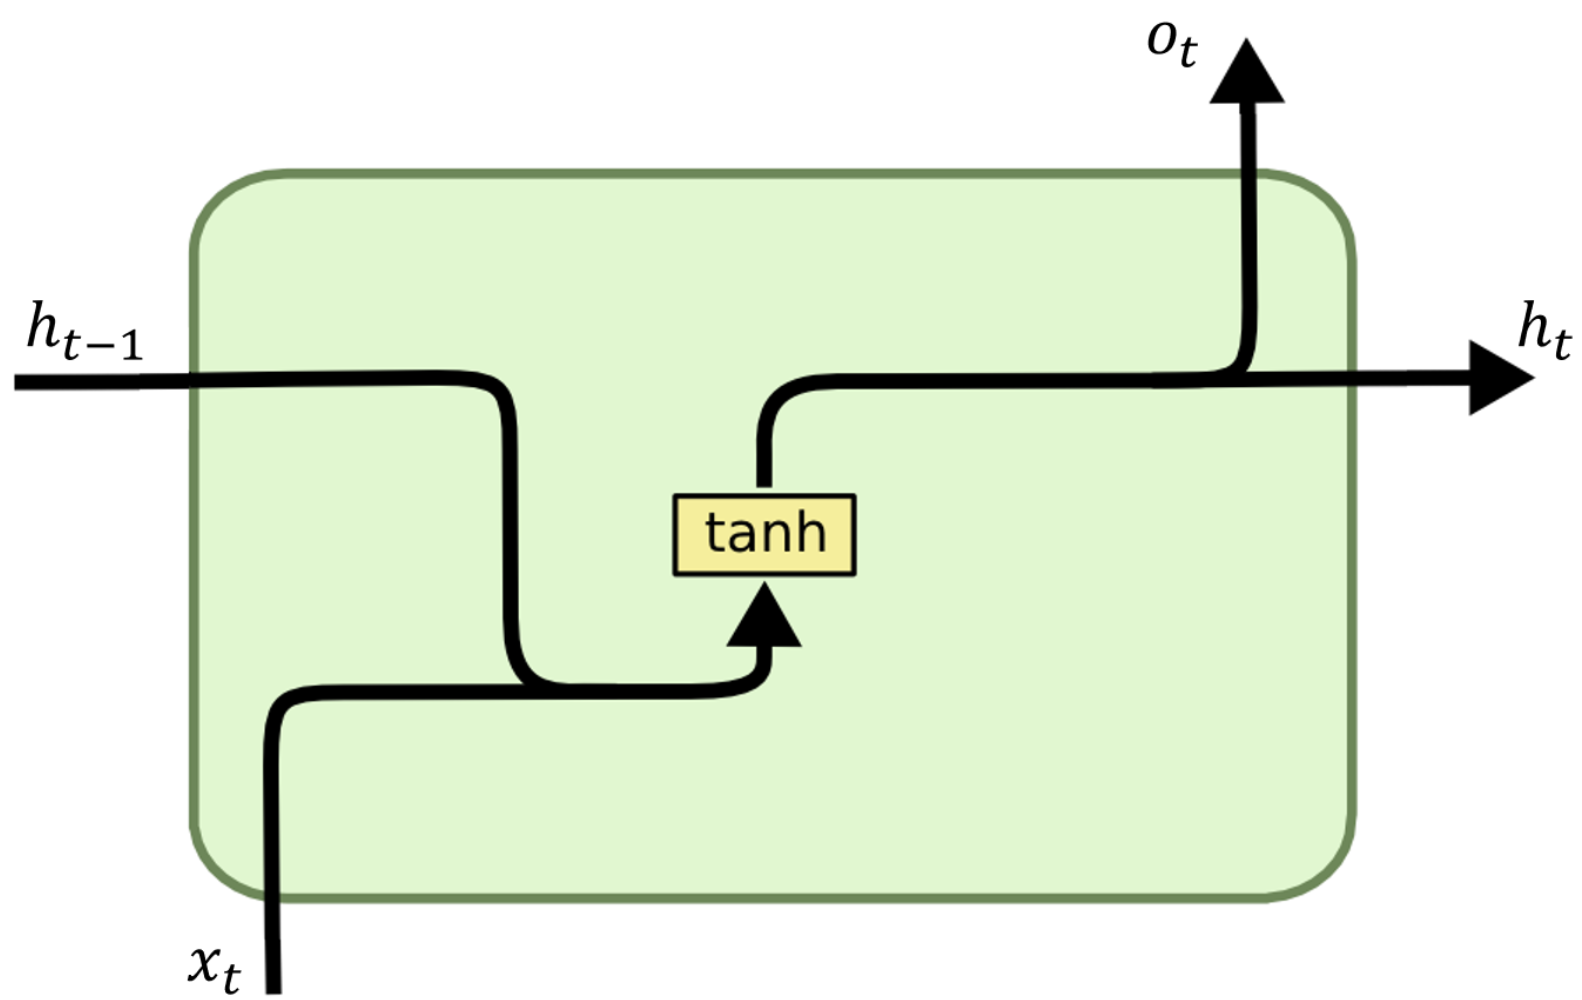
\includegraphics[scale=0.25]{img/rnn_basic_cell.png}
        \caption{A basic RNN cell}
    \end{figure}
    
\end{multicols}

\section{Long-Short Term memories (LSTM)}
The \textit{Long-Short Term memories (LSTM)} (\cite{hochreiter1997long}) memory cell was introduced in \citedate{hochreiter1997long} by \Citeauthor{hochreiter1997long}. 
If you consider an LSTM cell as a black-box, it can be used in practice as a basic cell, with the only difference that it performs much better. Another difference is that its state is split into \textbf{two vectors}: $\mathbf{h}_{(t)}$ that is the \textit{short-term state} and $\mathbf{c}_{(t)}$ (c $\to$ cell) which is the \textit{long-term state}. Now it is interesting to understand, \textbf{What is inside the box?}
The key idea behind this novel type of cell is that the network can learn what to store in the long-term state, what to forget and what to read from it in order to give the short-term state. The input $\mathbf{x}_{(t)}$ and the hidden state $\mathbf{h}_{(t)}$ are fed into four different \textit{fully connected layers}. They have different purposes:
\begin{enumerate}
    \item[\ding{202}] The main layer is the one which do have as output $\mathbf{g}_(t)$. This is nothing but the role charachterizing a basic cell, here the difference is that only most important part are retained in the long-term state.
    \item[\ding{203}] The other three layers have the role of \textbf{gate controllers}, since the have \textit{logistic activation} (see the figure below). Their outputs are convolved into element-wise multiplication operator such that if the output is 0s they close the gate, if they are 1s the gate are opened. More specifically: 
    \begin{itemize}
        \item The \textbf{forget gate} (controlled by $\mathbf{f}_{(t)}$) controls \textit{which part of the long-term state should be deleted}; 
        \item The \textbf{input gate} (controlled by $\mathbf{i}_{(t)}$) controls which part of $\mathbf{g}_{(t)}$ should be added to the long-term state; 
        \item the \textbf{output gate} (controlled by $\mathbf{o}_{(t)}$) controls which part of the long-state should be read and output in the term $\mathbf{h}_{(t)}$. In this case the output $\mathbf{\hat{y}}_{(t)}$ and $\mathbf{h}_{(t)}$ are coincident.
    \end{itemize}
\end{enumerate}
\vspace{-0.3cm}
\begin{figure}[H]
    \centering
    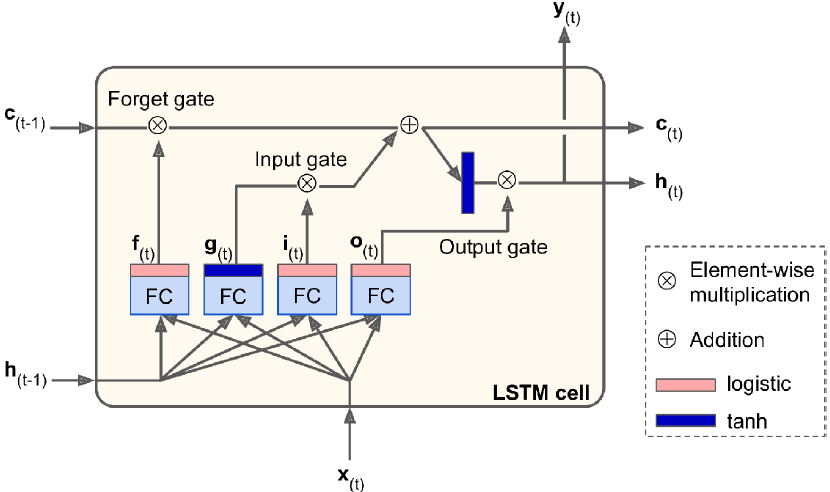
\includegraphics[scale=0.7]{img/LSTM.png}
    \caption{LSTM cell}
\end{figure}
\vspace{-0.3cm}
\noindent
An LSTM is able to recognize an important input (input gate) and store it (in the long-term state), until is needed (role of forget gate), and extract it whenever it is needed (role of the output gate). The equations (for a single instance) describing the LSTM cell are reported here: 
\begin{align}
    &\mathbf{i}_{(t)} = \sigma\big(
        \mathbf{W}_{xi}^T \mathbf{x}_{(t)}+
        \mathbf{W}_{hi}^T \mathbf{h}_{(t-1)} + \mathbf{b}_i    
    \big) \qquad \textsf{(\textbf{input gate} controller)}\\
    &\mathbf{f}_{(t)} = \sigma\big(
        \mathbf{W}_{xf}^T \mathbf{x}_{(t)}+
        \mathbf{W}_{hf}^T \mathbf{h}_{(t-1)} + \mathbf{b}_f    
    \big) \qquad \textsf{(\textbf{forget gate} controller)} \\
    &\mathbf{o}_{(t)} = \sigma\big(
        \mathbf{W}_{xo}^T \mathbf{x}_{(t)}+
        \mathbf{W}_{ho}^T \mathbf{h}_{(t-1)} + \mathbf{b}_o    
    \big) \qquad \textsf{(\textbf{output gate} controller)}\\
    &\mathbf{g}_{(t)} = \tanh\big(
        \mathbf{W}_{xg}^T \mathbf{x}_{(t)}+
        \mathbf{W}_{hg}^T \mathbf{h}_{(t-1)} + \mathbf{b}_g    
    \big) \quad \textsf{(basic cell output)}\\
    &\mathbf{c}_{(t)}= \mathbf{f}_{(t)} \otimes \mathbf{c}_{(t-1)} + \mathbf{i}_{(t)}\otimes \mathbf{g}_{(t)} \qquad \textsf{(long-term state)}\\
    &\mathbf{h}_{(t)}=\mathbf{y}_{(t)}=\mathbf{o}_{(t)} \otimes \tanh(\mathbf{c_{(t)}}) \qquad \textsf{(short-term state and output)}
\end{align}

\section{Gated Recurrent Unit (GRU)}
The \textit{Gated Recurrent Unit (GRU)} cell is a \textbf{simplified version} of the LSTM cell. Different studies has demonstrated that the performances are the same, this explains their growing popularity. 
Such a type of cell has been introduced in \citedate{cho2014learning} in the article \textit{\citetitle{cho2014learning}}, that also introduced the encoder-decoder network we have introduced so far. In the following we are going to mention the main simplifications:
\begin{enumerate}
    \item Long-term and Short-term states are merged into a single hidden state denoted with $\mathbf{h}_{(t)}$; 
    \item There is a single  \textbf{gate controller} called $\mathbf{z}_{(t)}$ for the \textit{forget} and \textit{input} gates. If $\mathbf{z}_{(t)}$ outputs a 1, the forget gate is open, and the input gate is closed (1-1=0) and viceversa.
    \item There is \textbf{no output gate}, the full state vector is output at every step. However there is a new controller gate $\mathbf{r}_{(t)}$ that decides which part of the state must be shown into the main layer $\mathbf{g}_{(t)}$.
\end{enumerate}
Here the equations are the following: 
\vspace{-0.5cm}
\begin{figure}[H]
    \centering
    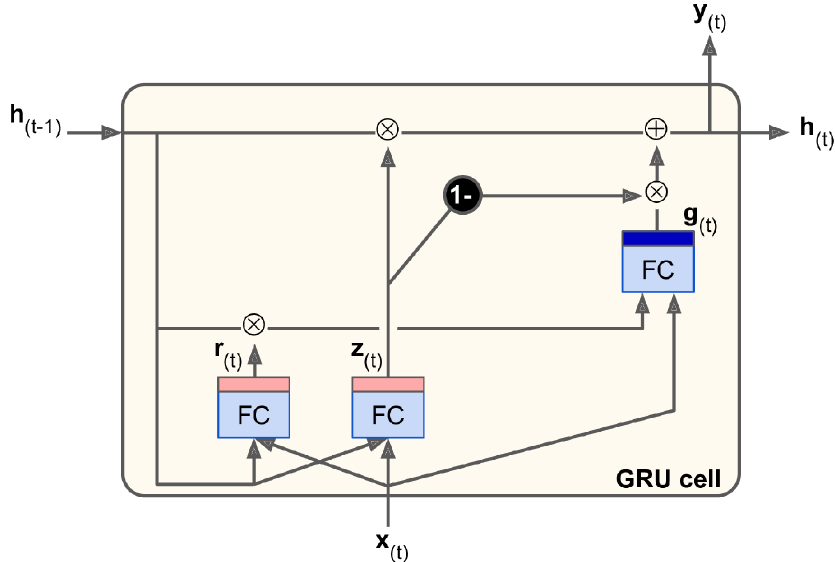
\includegraphics[scale=0.6]{img/GRU_cell.png} 
    \caption{A \textit{GRU cell}}
\end{figure}
\vspace{-1cm}
\begin{align}
    &\mathbf{z}_{(t)}=\sigma\big(
        \mathbf{W}_{xz}^T \mathbf{x}_{(t)}+
        \mathbf{W}_{hz}^T \mathbf{h}_{(t-1)}+
        \mathbf{b}_{z}
    \big)\\
    &\mathbf{r}_{(t)}=\sigma\big(
        \mathbf{W}_{xr}^T \mathbf{x}_{(t)}+
        \mathbf{W}_{hr}^T \mathbf{h}_{(t-1)}+\mathbf{b}_{r}
    \big)\\
    &\mathbf{g}_{(t)}=\tanh\big(
        \mathbf{W}_{xg}^T \mathbf{x}_{(t)}+
        \mathbf{W}_{hg}^T \big(\mathbf{r}_{(t)}\otimes\mathbf{h}_{(t-1)}\big)+\mathbf{b}_{g}
    \big)\\
    &\mathbf{h}_{(t)}=\mathbf{z}_{(t)}\otimes\mathbf{h}_{(t-1)} + \big(1-\mathbf{z}_{(t)}\big) \otimes \textsf{g}_{(t)}
\end{align}


\noindent
LSTM and GRU are the main reason behind the success of RNNs, however still there are problem with the short-term memory, moreover there is an hard time learningfor long patterns longer than 100 steps.

\begin{comment}
The process of image captioning involves several key steps, typically executed by a machine learning model. Here's a breakdown of the general steps:

### 1. *Image Preprocessing*
   - *Resize and Normalize*: The image is resized to a fixed dimension (if necessary) and normalized (adjusting pixel values to a certain range, typically between 0 and 1).
   - *Feature Extraction*: Convolutional neural networks (CNNs) or pre-trained models like ResNet, Inception, or VGG are often used to extract key visual features from the image, such as objects, backgrounds, and structures.

### 3. *Encoding the Image*
   - The visual features extracted from the image are then encoded into a compact, informative representation. This often involves using the output of the last layer of the CNN as a feature vector, which captures high-level information about the image.

### 4. *Caption Generation*
   - *Sequence Generation*: Using the encoded image features as input, a sequence generation model (often a Recurrent Neural Network (RNN), Long Short-Term Memory (LSTM), or a Transformer model) is used to generate the caption.
     - The model is trained on large datasets with corresponding image-caption pairs, so it learns to predict the most likely words or phrases based on the encoded image features.
   - The model generates the caption word by word, often starting with a special token like "start of sequence" and continuing until it predicts a "end of sequence" token.

### 5. *Postprocessing*
   - The generated caption may be refined by applying language rules to make it grammatically correct, coherent, and contextually appropriate.
   - Some models also add punctuation or handle plural/singular noun agreements.

### 6. *Final Caption Output*
   - The model produces a complete, coherent sentence (or set of sentences) that describes the image.

### Example Flow:
1. *Input Image*: A photo of a person with a dog in a park.
2. *Feature Extraction*: The CNN extracts features like "person," "dog," "park," "grass," etc.
3. *Caption Generation*: The LSTM or Transformer model takes the image features and generates a description like: "A person standing in a park with a dog on a leash."
4. *Postprocessing*: Ensuring the caption is grammatically sound.

This whole process allows AI systems to automatically generate textual descriptions for images, helping with accessibility, image search, and other applications.
\end{comment}

%--------------Attention models (II gruppo di slides)------------------
\section{Image captioning with RNN}
\begin{figure}
    \centering
    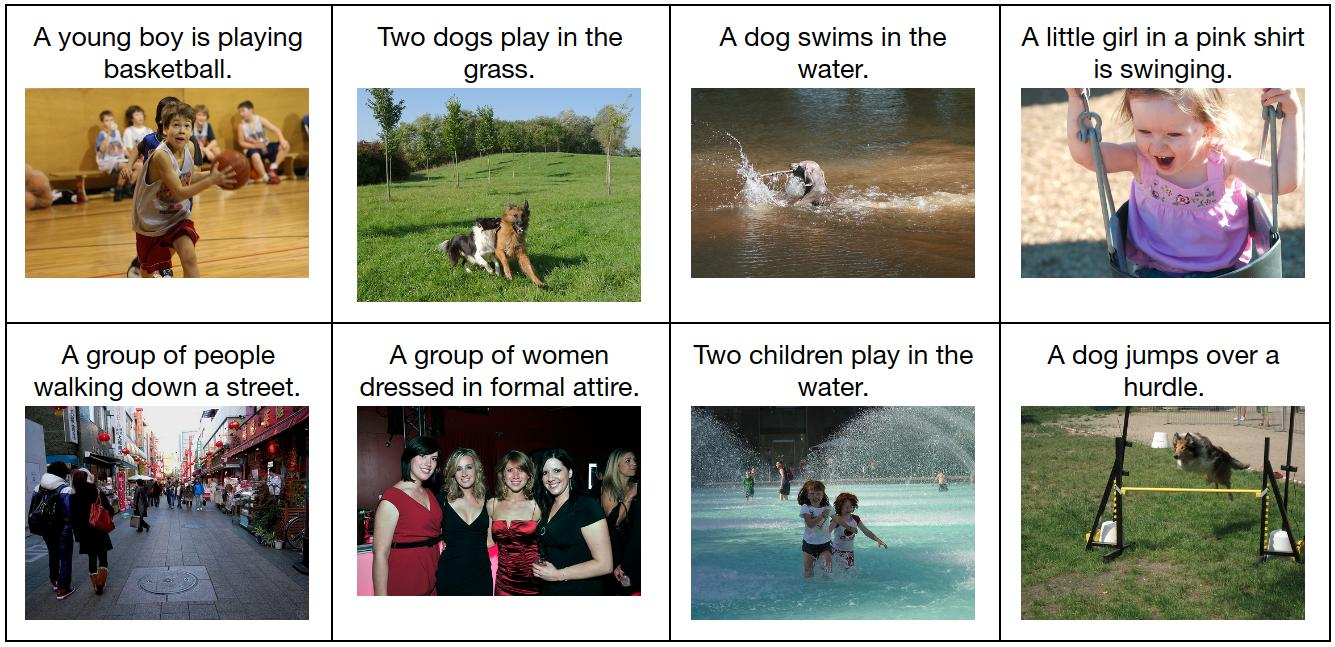
\includegraphics[scale=0.28]{img/img_caption.jpg}
    \caption{Example of image captioning}
\end{figure}
The \textbf{Image captioning} is a task that deals with \textbf{extracting a brief description (caption) given an input image}. This is a not so simple task which sees the colaboration between two different deep learning models: a convolutional network (ConvNet) for image classification (Inception, ResNet, VGG16...) with an RNN that is employed for generating the textual description. The general steps are: 
\begin{enumerate}
    \itemsep-0.2em
    \item \textsf{Image Preprocessing} The image is resized to a fixed dimension and normalized, a CNN is used to extract \textit{visual features} from the image;
    \item \textsf{Encoding the image} The visual features are encoded into a compact representation. This often involves using the \textit{last layer output as a feature vector}, which mainly captures the high level information about the image; 
    \item \textsf{Caption generation} Using the encoded image features as input, a sequence generation model (RNN, LSTM, GRU) is used to \textit{generate the caption}. The model generates the caption word by word, starting from a special <SOS> token and ending with another special token <EOS>. The model is  \textbf{trained} on large datasets with corresponding image-caption pairs, so it learns to predict the most likely words or phrases based on the encoded features vector.
\end{enumerate}

Let $v$ be the feature vector extracted from the CNN output, the hidden state equation is modified as follows in order to take into account the image features in the caption generation: 
\begin{equation*}
    \mathbf{h}_{(t)}=g\big(
        \mathbf{W}_{hh} \mathbf{h}_{(t-1)}+
        \mathbf{W}_{hx} \mathbf{x}_{(t)}+
        \mathbf{W}_{hi} \mathbf{v}+
        \mathbf{b}_h
    \big)
\end{equation*}
where $\mathbf{W}_{hi}$ is a new weight matrix accounting for the relationship between the hidden state and image features vector.

\begin{figure}[h]
    \centering
    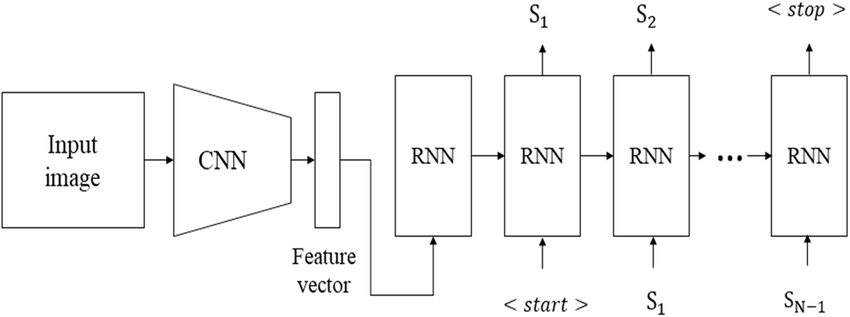
\includegraphics[scale=1.4]{img/img_caption_2.jpg}
    \caption{Architecture for image captioning}
\end{figure}

\section{Attention mechanisms}
Let us focus for a while on the neural machine translation task. We have seen that an encoder-decoder mechanism is used, moreover we have seen that using a bidirectional RNN is better for such a task. If we better analyze this process, we will understand that the path between the word to translate and the translated one is quite long. \\
\citeauthor{bahdanau2014neural} in the paper \cite{bahdanau2014neural}, introduced a technique by which allows the decoder to focus on the appropriate word to be translated. By using such a modified architecture, the encoder instead of sending only the final hidden state, it sends \textbf{all of its outputs to the decoder}. The decoder computes a weighted sum of such outputs by using some weights $\alpha_{(t,i)}$ for the $t$-th time step and  for the $i$-th encoder output. For example if
\begin{equation*}
    \alpha_{(3,2)} > \alpha_{(3,1)} > \alpha_{(3,0)}
\end{equation*}
this means that at the third time step the decode will pay much more \textbf{attention} on the term 2 which in this case is \textit{milk}. The weights $\alpha_{(t,i)}$ are produced by a small neural network which is called the \textbf{alignment model}\footnote{
    \textbf{Alignment model} comes from the fact that we are seeking a form of coherence (alignment) between the encoder's outputs and the decoder hidden state. The closer the encoding of the hidden state to a certain output, the higher the associated $\alpha$-weight.
} (or \textbf{attention layer}). How it can be seen this is made up of a \textbf{Time Distributed dense layer}\footnote{
    The layer is applied independently at each time step
} whose inputs are all the outputs from the decoder and the hidden state from the previous step-time. The \texttt{Dense Layer} outputs an \textit{energy score} for each encoder output which measures how \textit{well aligned} is that output with respect to the previous hidden state. The $\alpha$-weights are obtained using a softmax layer which is not time distributed. This attention mechanism is called \textit{Bahdanau attention} or \textit{concatenative attention}.

\begin{figure}
    \centering
    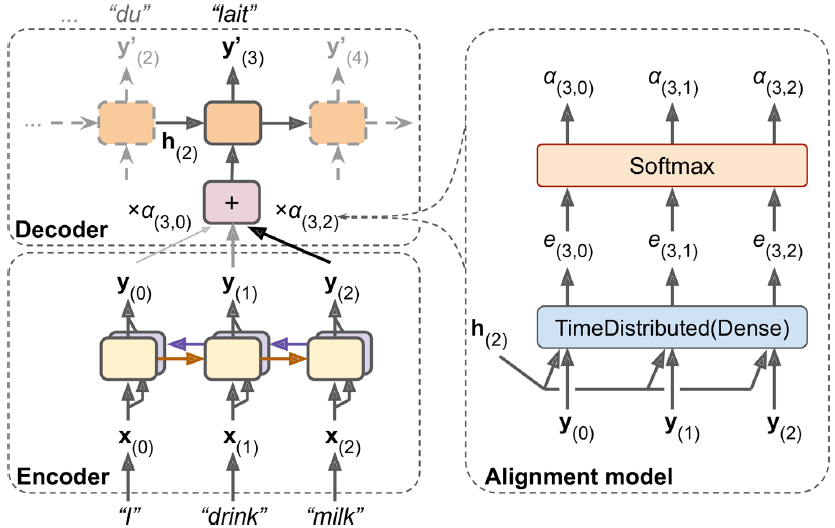
\includegraphics[scale=0.6]{img/attention_1.png}
    \caption{Encoder-Decoder with attention}
\end{figure}

Another mechanism which is called \textit{Luong attention} or \textit{multiplicative attention} is based on the \textbf{dot-product} between the the encoder's output and the \textbf{decoder previous hidden state}, this is a quite fair \textit{similarity measure}, since the dot product is related to a $\cos \theta$. The result is passed through a softmax which will compute the attention weigths.

\subsection{Image captioning with attention}
This is in general the same task we have seen before with the only difference that the attention mechanism enhances the performances of the model.\\
\noindent
Here some \textbf{feature vectors} are generated corresponding to different region of the image. These serve as the \textbf{values} and \textbf{keys} in the attention mechanism. \\ The \textit{Caption generation} also here occurs one word at a time, and  according to an RNN with attention or a transformer. Here the hidden state plays the role of \textbf{query} in the attention mechanism. At each time step \textbf{attention weights} are computed for each image region highlighting the regions most relevant to the current word.

\subsubsection{Attention weight calculation}
The model calculates attention scores using dot product between the query (current RNN hidden state) and the keys (image features). The scores are passed through a softmax in order to obtain the attention \textbf{attention weights}.

\subsubsection{Context vector}
The weighted sum of image features, using attention weights, creates a \textbf{context vector}, this combined with the hidden state of the RNN, is used to predict the next word.

\begin{figure}
    \centering
    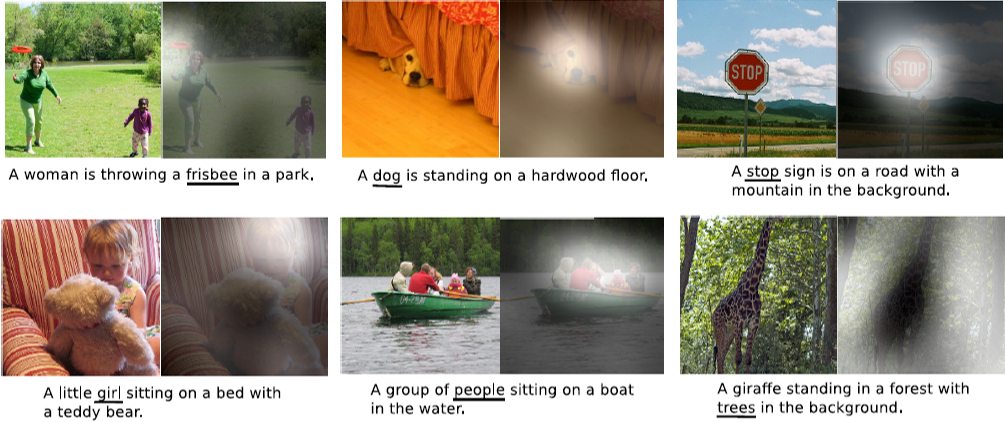
\includegraphics[scale=0.5]{img/img_caption_3,jpg.png}
    \caption{Examples of image captioning with attention}
\end{figure}

\subsection{Visual question answering}
\begin{figure}[h]
    \centering
    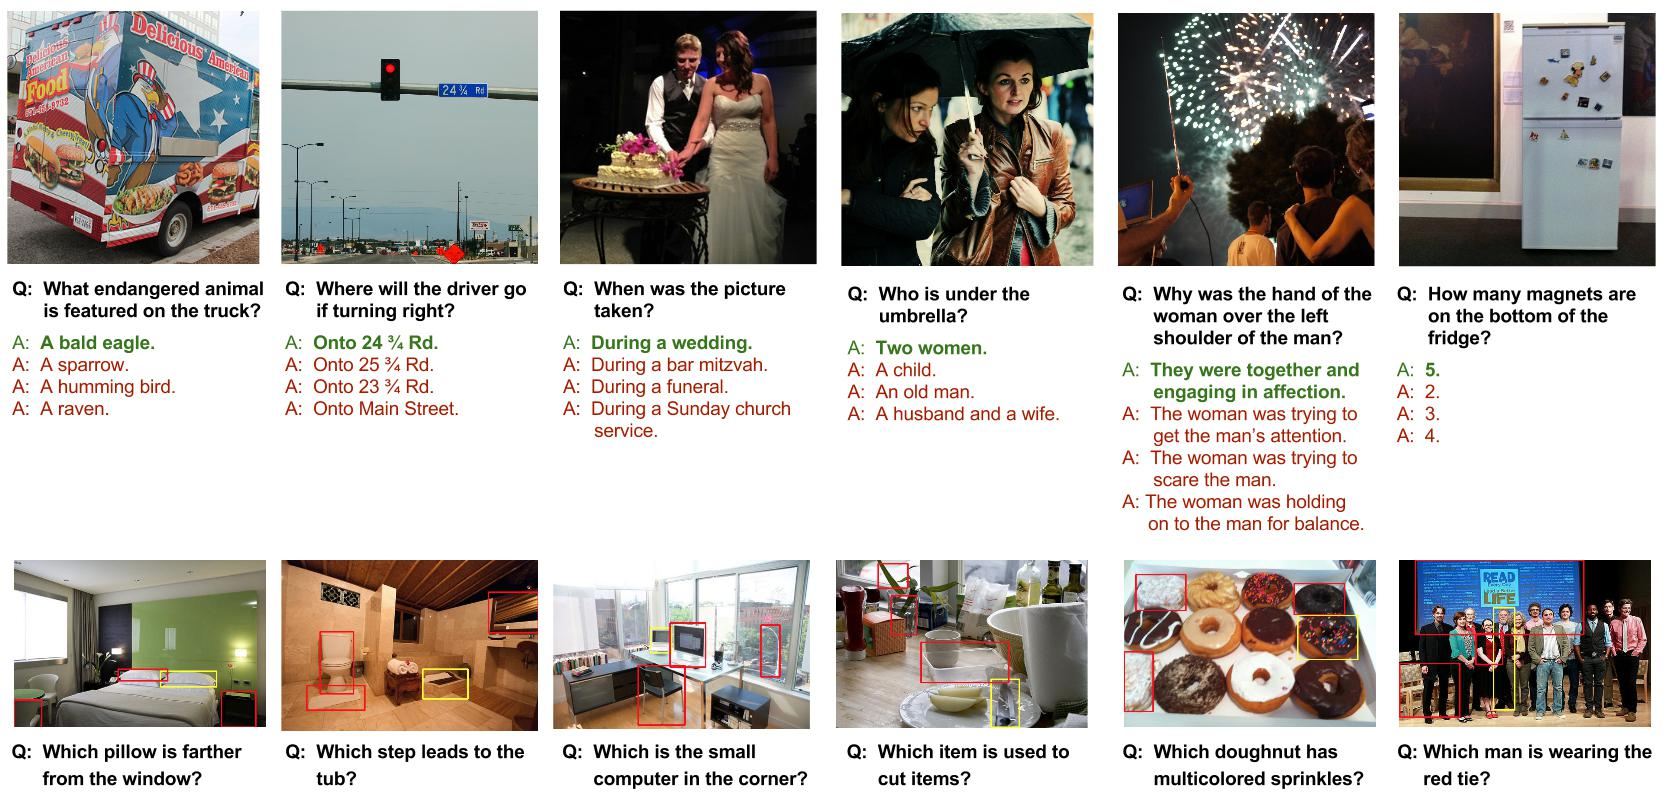
\includegraphics[scale=0.2]{img/visual7w.jpg}
    \caption{\textit{Visual question answering example}}
\end{figure}
The task of \textbf{Visual Question Answering (VQA)} is a complex deep-learning task, that sees the fusion of visual task with textual tasks. The input of the model is an image with a related question. For example an image of a car, and a question \textit{what color is the car?} The output is in textual form (for example \textit{red}). There are three main phases: 
\begin{enumerate}
    \itemsep-0.2em
    \item \textsf{Feature Extraction} the visual features are extracted using a ConvNet, the textual ones using a model like RNN with attention or a transformer.
    \item \textsf{Multimodal fusion} The features are combined by using some form of element-wise multiplication, dot product...
    \item \textsf{Answer generation} Here there is a classifier that predicts the answer by using a predefined set of answers for VQA.
\end{enumerate}

\subsubsection{Attention in VQA}
Attention mechanisms are crucial in VQA to focus on relevant parts of the image or question:
\begin{itemize}
    \itemsep-0.2em
    \item \textbf{Visual Attention}: identifies specific regions in the image relevant to the question. For example, when asked, "What is the person holding?", the model attends to the hands and objects in the image; 
    \item \textbf{Question Attention}: highlights important words or phrases in the question to guide the visual attention.
    \item \textbf{Multimodal Attention}: dynamically attends to both the image and the question simultaneously, ensuring the model aligns the two modalities effectively.
\end{itemize}
\noindent
Famous papers on VQA are: 
\begin{itemize}
    \itemsep-0.2em
    \item \citeauthor{antol2015vqa} \citetitle{antol2015vqa}, \citeyear{vqa}, \cite{antol2015vqa} 
    \item \citeauthor{zhu2016visual7w} \citetitle{zhu2016visual7w}, \citedate{zhu2016visual7w}, \cite{zhu2016visual7w}
\end{itemize}


\section{Attention is all you need: \textit{Transformer} architecture}
In a \citedate{vaswani2017attention} paper (\cite{vaswani2017attention}, \citetitle{vaswani2017attention}), some Google researchers proposed a mechanism which significantly improved the NMT field in which no recurrent or convolutional layers was used, only \textbf{attention mechanism} together with fully connected, embedding, normalization layers and few other pieces of data. The transformer architecture is presented in the \Cref{fig:transformer_arch}. \\
The left part of the figure is the \textbf{encoder} which receives the input as \textit{word IDs}, these are passed through an embedding lookup, the top part of the encoder is stacked $N$ times.\\

\noindent
The right part of the figure represents the \textbf{decoder} which during the training is fed with the target sequence and with the output from the encoder, similarly than the other encder-decoder models, the output is a probability distribution over all of the words of a given vocabulary.\\

\noindent
Looking more closely there are 2 embedding layers, $5\times{N}$ skip connections, $2\times{N}$ feed-forward layers composed of two dense layers which are not-recurrent and so \textbf{time-distributed} so that each word is treated independently from the others.\\
Now, how can be avoided the presence of recurrent layers? That is how can a word be processed indepently from the others? At this point two novel elements comes into play:
\begin{itemize}
    \itemsep-0.2em
    \item \textsf{Multi-Head attention module} such a module encode in a compact way all the relationship between a word in the sentence and all the others. For example in the sentence \textit{They welcomed the Queen of the United Kingdom}. The output of this layer for the word "Queen" will have higher weights for the words "United" and "Kingdom" than for other words. This mechanism is called \textbf{self-attention} (since the sentence is paying attention to itself); the Multi-head attention module is based on the \textbf{scale dot-product attention}.
    \item \textsf{Positional embedding module} The multi-head attention module does not keep track of the position of a certain word in a given sentence from the mini-batch, this is an important information for the Transformer to be processed. For this reason a \textit{positional embedding vector} is added to the word embedding. Such added vector allows to the model to keep track about absolute/relative positions of the words within a sentence.
\end{itemize}


%\subsection{Positional Embeddings}

\subsection{Scaled Dot-product attention}
A fundamental brick for Transformer is the \textbf{scaled-dot product attention}, this allows us to focus on the most relevant part when meaking decision.

\begin{equation}
    \text{Attention}(\mathbf{Q},\mathbf{K},\mathbf{V})=
    \text{softmax}\bigg(
        \frac{\mathbf{Q}\mathbf{K}^T}{\sqrt{d_{keys}}}
    \bigg)\mathbf{V}
\end{equation}
where the components are:
\begin{itemize}
    \item \textbf{Query (Q)} A vector for each word embedding that represents what we are looking for.
    \item \textbf{Key (K)} Is a reference point, these determine how relevant different parts are to the query, they represents all the "things" we can focus on
    \item \textbf{Value (V)} is the actual content that we want to extract after deciding where to focus (eg. the meaning of the most relevant word).
\end{itemize}

\noindent
\textbf{Q, K, V} are obtained by applying three separate learned linear transformations to the input embeddings. In particular they are obtained through the multiplication by using learnable weight matrices $W^Q, W^K, W^V$. Then they are obtained as:
\begin{equation}
    \mathbf{Q}=\mathbf{X} W^Q \quad 
    \mathbf{K}=\mathbf{X} W^K \quad
    \mathbf{V}=\mathbf{X} W^V
\end{equation}
 



\subsection{Multi-head Attention layer}
When we want to improve the attention mechanism in Transformers, \textbf{Multi-head attention} is used, here the model computes multiple attention in parallel. In particular \textbf{each head} learns  to focus on different parts of the input. This leads to an enhancement in the general performances. Here there are the steps behind the multi-head attention mechanism: 
\begin{enumerate}
    \item \textbf{Splitting the input} Here the input embeddings $X$ are transformed into Query, Key and Value matrices by projecting X on a certain subspace defined by the learnable matrices $W^Q$, $W^K$, $W^V$.
    \item \textbf{Parallel Attention heads} In this context different weight matrices are used for each head. Moreover if we have $h$ heads and the dimension of the embeddings is $d$, the $i$-th head works on vectors of dimension $d/h$, that is:
    \begin{equation}
        \text{head}_i=\text{Attention}(\mathbf{Q}W_i^Q, \mathbf{K}W_i^K, \mathbf{V}W_i^V)
    \end{equation}
    \item \textbf{Concatenation of heads} the output of the $h$ heads is concatenated as follows:
    \begin{equation}
        \text{Concat}=[\text{head}_1,\text{head}_2,...,\text{head}_h]
    \end{equation}
    so that the resulting matrix has dimensione $N\times{d}$ where $N$ is the batch size.
    \item \textbf{Final linear transformation} The final attention result is obtained as: 
    \begin{equation}
        \text{Multihead}(Q,K,V)=\text{Concat}=[\text{head}_1,\text{head}_2,...,\text{head}_h]W^O
    \end{equation}
    with $W^O$ learnable matrix.
\end{enumerate}

\begin{figure}
    \centering
    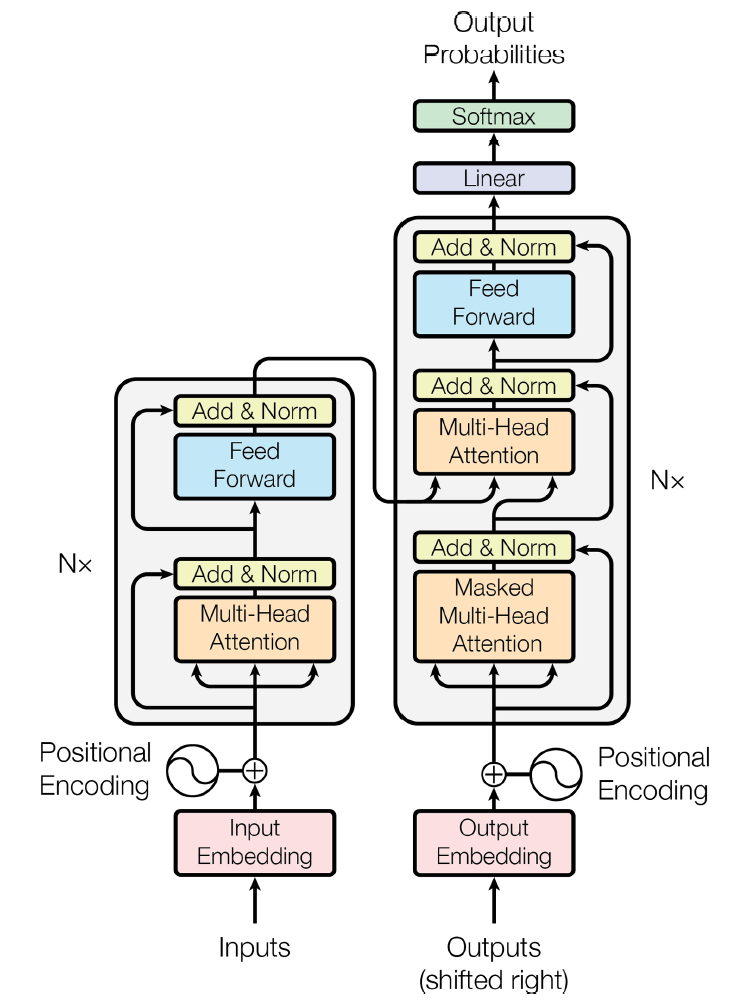
\includegraphics[scale=0.8]{img/transformer_archs.png}
    \caption{The \textbf{Transformer} architecture}
    \label{fig:transformer_arch}
\end{figure}

\begin{multicols}{2}
    \begin{figure}[H]
        \centering
        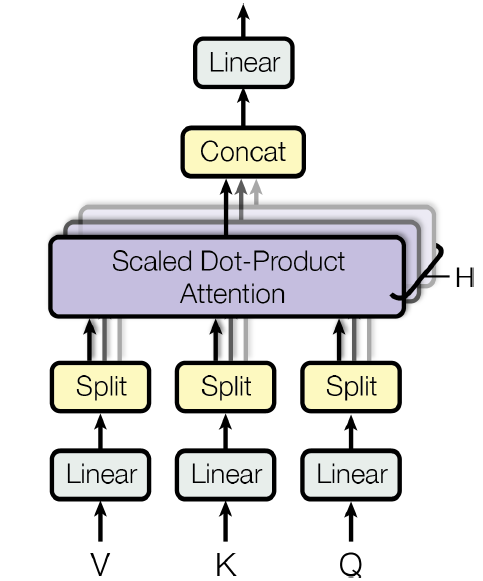
\includegraphics[scale=0.7]{img/multi_head.png}
        \caption{Architecture of the \textit{Multi-Head layer}}
    \end{figure}

    \begin{figure}[H]
        \centering
        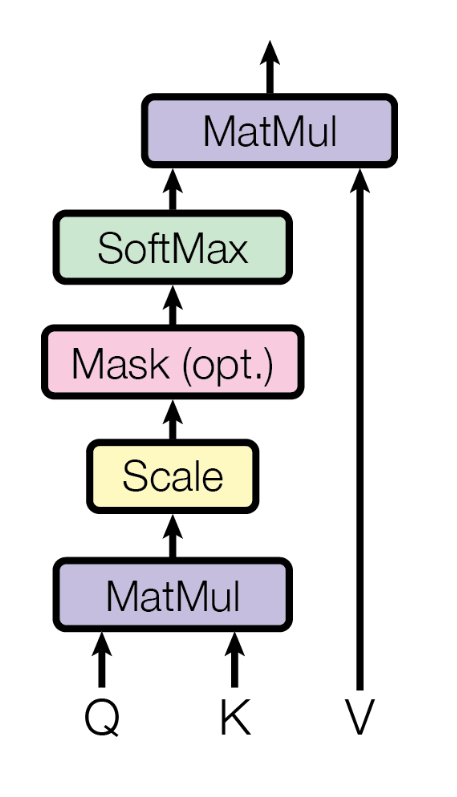
\includegraphics[scale=0.5]{img/scaledDotProduct.png}
        \caption{Scaled-dot product attention}
    \end{figure}
\end{multicols}



\section{Transformers vs RNN}
In order to conclude this chapter we provide a comparison between Transformers and RNN in term of mechanisms, performance and so on. 

\renewcommand{\arraystretch}{1.5}
\setlength{\tabcolsep}{8pt}

\begin{longtable}{|>{\raggedright\arraybackslash}p{3.5cm}|>{\raggedright\arraybackslash}p{6cm}|>{\raggedright\arraybackslash}p{6cm}|}
\hline
\textsc{Aspect} & \textsc{Transformers} & \textsc{RNNs} \\ \hline
\endfirsthead
\hline
\textsc{Aspect} & \textsc{Transformers} & \textsc{RNNs} \\ \hline
\endhead
\hline
\endfoot
\hline
\endlastfoot

\textbf{Architecture} & Uses self-attention to process input sequences in parallel. & Processes sequences step-by-step using recurrence, one token at a time. \\ \hline

\textbf{Sequence Processing} & Processes the entire sequence simultaneously (parallel processing). & Sequentially processes tokens, one after another. \\ \hline

\textbf{Memory Handling} & Handles long-range dependencies effectively using self-attention. & Struggles with long-term dependencies due to vanishing/exploding gradients. \\ \hline

\textbf{Parallelism} & Fully parallelizable; faster training and inference. & Sequential nature prevents parallelism; slower training and inference. \\ \hline

\textbf{Positional Information} & Requires explicit positional encoding (e.g., sinusoidal or learned embeddings). & Naturally handles positional information through sequence order. \\ \hline

\textbf{Variable-Length Sequences} & Easily handles variable-length sequences with masking. & Handles variable-length sequences natively but requires padding for training. \\ \hline

\textbf{Long-Term Dependencies} & Excellent; attends to all tokens regardless of their distance. & Poor; performance degrades with longer dependencies (though improved with LSTMs/GRUs). \\ \hline

\textbf{Expressiveness} & Highly expressive due to self-attention and multiple heads. & Limited by step-by-step processing and simpler architectures. \\ \hline

\textbf{Convergence} & Faster convergence due to parallelism and better gradient flow. & Slower convergence due to sequential processing and gradient challenges. \\ \hline

\textbf{Scalability} & Scales well to large datasets and models (e.g., GPT, BERT). & Struggles to scale efficiently to large datasets. \\ \hline

\textbf{Sequence Length} & Handles long sequences effectively with global attention. & Performance degrades significantly for long sequences. \\ \hline

\textbf{Applications} & 
State-of-the-art in NLP tasks (e.g., translation, summarization). Emerging use in vision (Vision Transformers). & 
Previously dominant in NLP. Common in time-series tasks but rare in vision applications. \\ \hline

\textbf{Strengths} & 
\begin{itemize}
    \item Parallel processing speeds up training and inference.
    \item Captures long-term dependencies well.
    \item Scales effectively to large datasets.
    \item Adapts well to different modalities (text, images, audio).
\end{itemize} & 
\begin{itemize}
    \item Naturally processes sequences step-by-step.
    \item Compact models are resource-efficient.
    \item Implicitly handles positional information.
\end{itemize} \\ \hline

\textbf{Weaknesses} & 
\begin{itemize}
    \item Quadratic complexity (\(O(N^2)\)) in self-attention can be costly for long sequences.
    \item Requires explicit positional encoding.
    \item High memory and computational requirements.
\end{itemize} & 
\begin{itemize}
    \item Slow training due to sequential bottlenecks.
    \item Gradient issues (vanishing/exploding) hinder long-term dependency modeling.
    \item Limited expressiveness compared to Transformers.
\end{itemize} \\ \hline

\textbf{Best Use Cases} & 
\begin{itemize}
    \item Long sequences and large datasets.
    \item NLP tasks (e.g., machine translation, summarization).
    \item Tasks requiring long-term dependency modeling.
\end{itemize} & 
\begin{itemize}
    \item Small-scale, sequential tasks (e.g., time-series forecasting).
    \item Applications where resources are limited.
\end{itemize} \\ \hline

\end{longtable}

